\section{Experiments \& Deployment}\label{sec:experiments}

\begin{figure}[h]
    \centering
    \begin{subfigure}{0.49\textwidth}
    \centering
    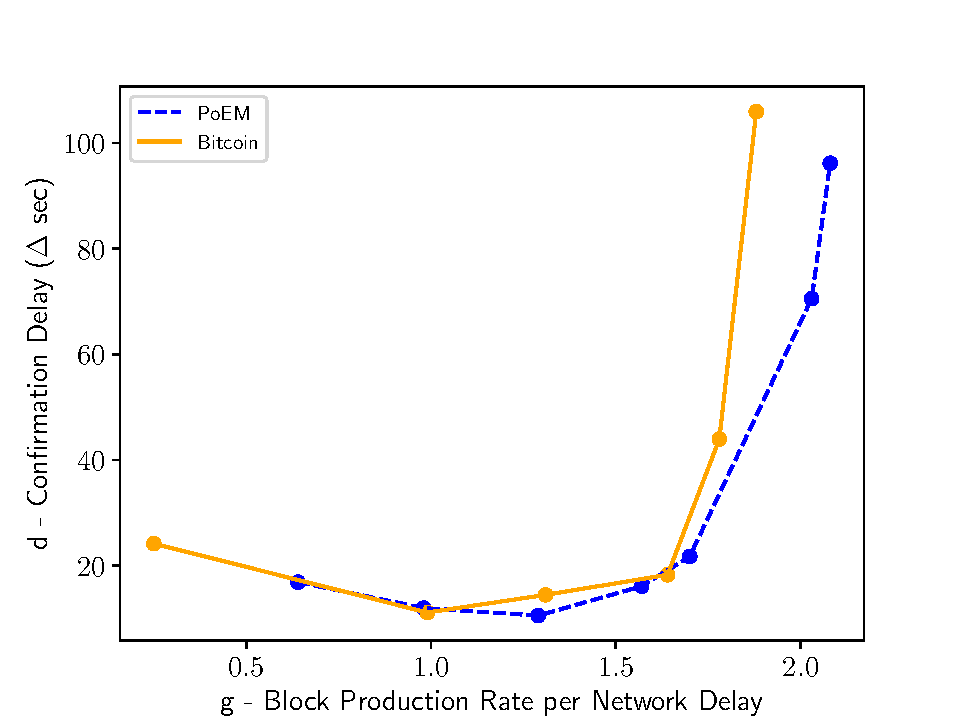
\includegraphics[width = 0.8\textwidth]{figures/dvsg.pdf}
    \caption{$d$ vs $g$}
    \label{fig:dvsg}
    \end{subfigure}
    \begin{subfigure}{0.49\textwidth}
    \centering
    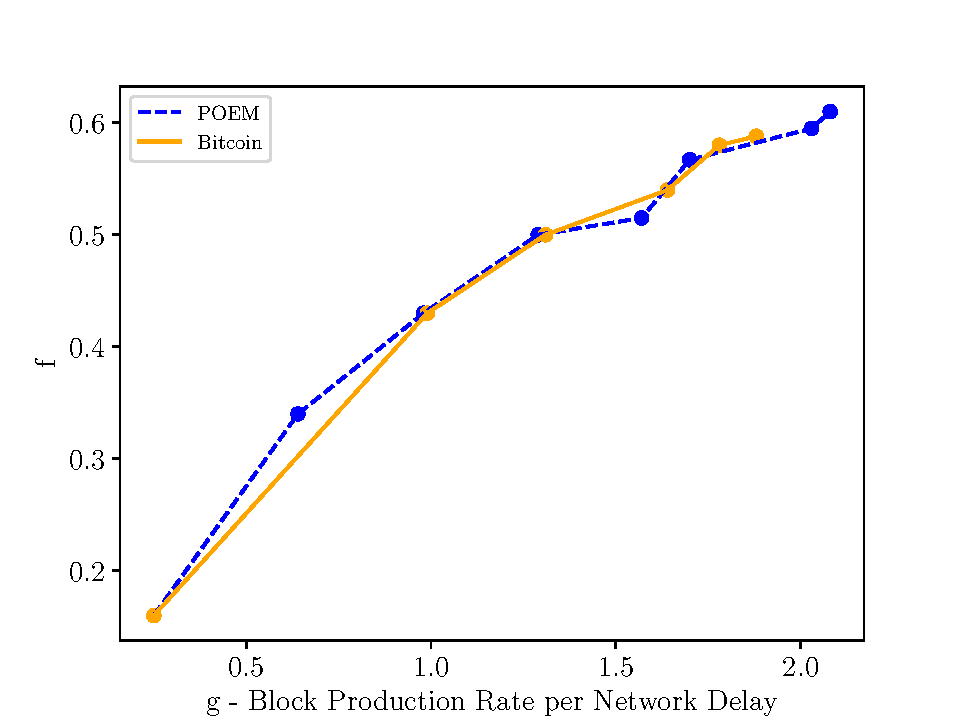
\includegraphics[width = 0.8\textwidth]{figures/fvg.pdf}
    \caption{$f$ vs $g$}
    \label{fig:fg}
    \end{subfigure}
    \caption{(a) Confirmation delay $d$ (measured in network delay $\Delta$ units) vs. the block production rate $g$. PoEM typically demonstrates lower confirmation delay for any given value of $g$, and the difference becomes more pronounced at large $g$. (b) The relationship between the honest block production rate $g$ and the honest chain growth rate $f$ for Bitcoin and PoEM.}
    \label{fig:results}
\end{figure}

In this section, we report on a real-world implementation and deployment of our
protocol, and experimental measurements illustrating the concrete improvements
in latency and throughput as compared to vanilla Bitcoin.

\subsection{Real-world Deployment}

We have implemented and deployed PoEM in a real-world permissionless peer-to-peer
setting\footnote{
    The source code resides in the following anonymized repositories:
    \begin{enumerate}
        \item \url{https://anonymous.4open.science/r/go-quai-228B/}
        \item \url{https://anonymous.4open.science/r/go-quai-3FB2}
        \item \url{https://anonymous.4open.science/r/go-quai-8610}
        \item \url{https://anonymous.4open.science/r/go-quai-DCB6}
        \item \url{https://anonymous.4open.science/r/simulation-0549}
        \item \url{https://anonymous.4open.science/r/quai-cpu-miner-7065}
    \end{enumerate}
}.
The deployment is on a testnet that has been continuously operating for
four months. During this period, the network generated over 7.5 million blocks
with participation from
more than 2000 miners/node operators from the community. Moreover, PoEM has facilitated the
confirmation of over 500 million testnet transactions. This deployment maintained an
average hash rate exceeding 50GH/s using the ProgPoW~\cite{progpow} hash algorithm.
The network participants computed more than 51 petahashes in 4 months.
The network operated in a variable difficulty and bias setting with the difficulty
varying between 18 and 790 billion and $\gamma$ varying between 32 and 38.

\subsection{Experimental Methodology}

We ran multiple simulations
in order to ascertain the optimal configuration for
operating both Bitcoin and PoEM in order to achieve the minimum confirmation delay.
We simulated an artificial network delay of $\Delta$ (measured in seconds) in the
communication between the honest parties in order to indirectly control the honest
block production rate $g$, measured in blocks per network delay. We define $g$ to
be the number of valid blocks cumulatively produced by the honest parties in one
network delay on average, including blocks that were subsequently abandoned
(following the terminology in~\cite{eiar}). This corresponds to the average number of
successful honest random oracle queries per network delay.
In the meantime,
we kept the mining target $T$ constant throughout the simulations (instead of varying
the network delay $\Delta$ and keeping $T$ constant, we could have, equivalently, kept
$\Delta$ constant and varied the target $T$). The target $T$ was not dynamically adjusted
during the simulation, in order to mimic the static nature corresponding to our theoretical
analysis.
Our goal was to plot the confirmation delay $d$ (in seconds) as a function of the
block production rate $g$ for both systems.

All executions included exactly
$n = 49$ parties, of which $t = 12$ were adversarial and $n - t = 37$ were honest.
The adversarial ratio was $\beta = \frac{t}{n} = 0.244$.
The honest parties ran the honest code of Bitcoin or PoEM respectively.
We fixed the adversarial strategy to be the private mining attack, which was
proven~\cite{eiar} to be the best possible attack against Bitcoin in the
continuous-time domain~\cite{bitcoin-made-simple}. This means that the network
began with a genesis block given to all honest and adversarial parties. The adversary
then mined blocks in private on her own chain, whereas the honest parties mined
their own blocktree without intervention by the adversary, following the heaviest chain
rule (in Bitcoin) or the most intrinsic work rule (in PoEM) respectively. To emulate the puppetmaster
nature of the adversary, we imposed no artificial network delay for the adversary.
On the contrary, every honest message was artificially delayed by exactly the maximum
delay bound $\Delta$.

Simulations were run on 49 virtual machines in Google Cloud all co-located in
the same data center. The configuration of the nodes used was 4 CPU cores, 4
GB of RAM, with a 10 GB SSD running Ubuntu 22.4. The honest party
had an artificial network delay between 100-1000ms (to allow for simulating varying
$g$). This delay was achieved by adding a \texttt{sleep} prior to every block message
broadcast. The adversary's network delay was only the inherent delay in communication
between virtual machines and was <5 ms. The tests were coordinated using Ansible and the
machines were given 2 minutes to peer with each other and stabilize at the beginning of
each test.
Both Bitcoin and PoEM were run on the same codebase,
with the exception of the appropriate modification to the proof-of-work inequality.

We ran each simulation until one of the honest parties managed to obtain a chain of
length $200$ blocks, at which point the simulation was halted and its lifetime $L$
(in units of $\Delta$) was measured. We recorded $g$ for that simulation as the number
of honest blocks produced divided by $L$ to find the average number of honest blocks
produced per network delay (regardless of whether they were ultimately abandoned or not).

For Bitcoin, at every block height
$1, \ldots, 200$ that appeared in the simulation, we recorded a flag indicating whether
the honest parties or the adversary was ahead. For each configuration of $g$, we
repeated the simulation $100$ times in a Monte Carlo fashion, and chose the value
$k^*$ to be the block height such that at least $90\%$ of the Monte Carlo simulations
indicated that the honest parties were ahead of the adversary from height $k^*$
onwards. This corresponds to accepting a probability of Common Prefix failure of
up to $10\%$.
We calculated the average honest chain growth rate $f$ as $f = L / 200$
(noting that $f \leq g$ and $0 \leq f \leq 1$, roughly following the terminology
of the Analysis section, and observing that, due to the heaviest chain rule,
the chain can grow no more than $1$ block per network delay when the honest
parties are operating alone).
The confirmation delay ($d$) for each configuration $g$ was obtained by dividing
this $k^*$ by $f$ to calculate the time needed to get $k^*$ blocks on average.

In PoEM's case, at every $\work$ point in intervals of $\gamma + \frac{1}{\ln2}$
(corresponding to the expected amount of work per valid block),
namely $\gamma + \frac{1}{\ln2}, 2\left(\gamma + \frac{1}{\ln2}\right), \ldots, 200\left(\gamma + \frac{1}{\ln2}\right)$.
For each of those $\work$ points, we record a flag indicating whether the honest
parties or the adversary first mined a chain with at least that amount of work.
Similar to the Bitcoin experiments, we ran $100$ Monte Carlo simulations and
calculated $k^*$ to be the $\work$ point such that at least $90\%$ of the
Monte Carlo simulations indicated that the honest parties were ahead of the
adversary from that $\work$ point onwards. The confirmation delay ($d$) for
each configuration $g$ was obtained by dividing this $k^*$ by $\frac{f}{\gamma + \frac{1}{\ln2}}$
to calculate the time needed to get $k^*$ work on average.

\subsection{Experimental Results}

Figure~\ref{fig:results}(a) illustrates the evolution of $d$ across different $g$ values. We
identified the best operating conditions for a protocol as the point where the
confirmation delay is minimized. In our simulations, Bitcoin achieved its lowest
delay of $25.58 \Delta$ at a block rate of $g=0.98$. On the other hand, at the same
$g$, PoEM reached the minimal delay of $18.29 \Delta$ operating with
$\gamma=10$. This means for the configuration minimizing the delay of each protocol,
PoEM had a $\frac{25.58 - 18.29}{25.58} = 28.5\%$ lower confirmation delay as compared to Bitcoin.

When either system operates at higher block production rate $g$, the honest chain
grows faster ($f$ also increases), but the confirmation delay $d$ increases as well.
We found that the relationships between $g$ and $f$ in Bitcoin and PoEM are
comparable (Figure~\ref{fig:results}(b)). However, for a given delay, PoEM can
safely operate at a higher block production rate $g$ than Bitcoin, yielding an
operation point with a higher honest chain growth rate $f$. In particular, we
found that, for example at $d = 25.6\Delta$, Bitcoin gives a chain growth rate
of $f = 0.43$, whereas PoEM gives a chain growth rate of $f = 0.5$, marking a
$16.3\%$ improvement in transaction throughput.
% Specifically, PoEM increases $f$ from 0.43 to 0.5, marking a 16.3\%
% improvement, for a comparable confirmation delay (Bitcoin($d=25.6$),
% PoEM($d=27.4$))